\chapter{System Design}
\label{chapter:system_design}

We want to present our system design in this chapter. We will outline the requirements that our system must achieve, as well as the design choices we took to accomplish so. 
Then, we will discuss the architecture of our system. 

\section{System Requirements}
We must first establish the requirements for our system before we can begin designing it. Our purpose is to detect heavy hitters in an ML-hybrid and completely time-aware~\cite{campos2014time} setting.
The following criteria are specified: 

\begin{enumerate}
    \item \emph{ML-hybrid~\cite{mohan2019effective} frequency estimation system} Our system should integrate machine learning models into algorithm design. 
    
    \item \emph{Efficient Heavy-Hitter detection} Our system should excel at identifying traffics with top counts.
    
    \item \emph{The tracking and data are both dynamic~\cite{widanagamaachchi2012interactive}} Our system should be able to address concept drift.
    
    \item \emph{Full information modeled but Heavy-Hitters prioritized} Our system should represent the same information in a combination of more latent (diffused) representation on lower-importance items (bottom) and more explicit representation on higher-importance items (top).

\end{enumerate}

\section{Design Choices}
To meet the criteria, we present the following design choices. 

\begin{enumerate}
    \item We bring learning-based~\cite{chen2014deep} streaming techniques into frequency estimation. Our algorithms use a learning process that allows them to exploit data features without being restricted to a specific pattern or prior knowledge of the attribute.  
    
    \item Instead of solely estimating frequency like Learned Sketch does, we transform the regression model into the classification model. Based on the counts output, we add layers on the top to acquire the probabilities of belonging to the top items and bottom items. To better evaluate the model performance, we combine AUC/F1 metric with MSE to not only monitor how well the model predicts counts, but also how accurately it detects the top hits. We also assign different weights to classes of 'top' and 'bottom' since we care mostly about the heavy hitters.
    
    \item We try to eliminate the most relevant examples to learn on, and go further by modeling importance in an explainable manner. We introduce a priority which is only partially inferred: instead of feeding the ground-truth counts as labels to the network, as they currently do, we feed the counts (the output of sketches) that we get from the whole system.
    
    \item We apply incremental~\cite{wu2019large} and online algorithms to the model training, since they continuously incorporate information into the model. The system is learning and updating as long as the new information is provided, it can quickly adapt to new information and gain insight into how important that new information is. That's why it is adaptive~\cite{wu2019real} and can effectively deal with concept drift. 
    
    \item We want to use the top k extraction module as a means to get gradually less global and more specific. We encode the top-k functionality directly in the neural network, alternated with deep layers. By doing so, we design a pyramid of top-k as pooling layers. As a result, we are able to represent items from more latent (down; full distribution modeled) to more explicit (up; only top modeled). 
    
\end{enumerate}

\section{System Workflow}

This section will describe our system's workflow. Our scheme is broken down into four components: i) RNN-based learned oracle, ii) optimizing performance of regression and classification, iii) importance-optimized model training including relabeling and semi-supervised learning, iv) top k pyramid pooling. 

\subsection{Learned Oracle Flow}

\begin{figure}[htbp]
\centering
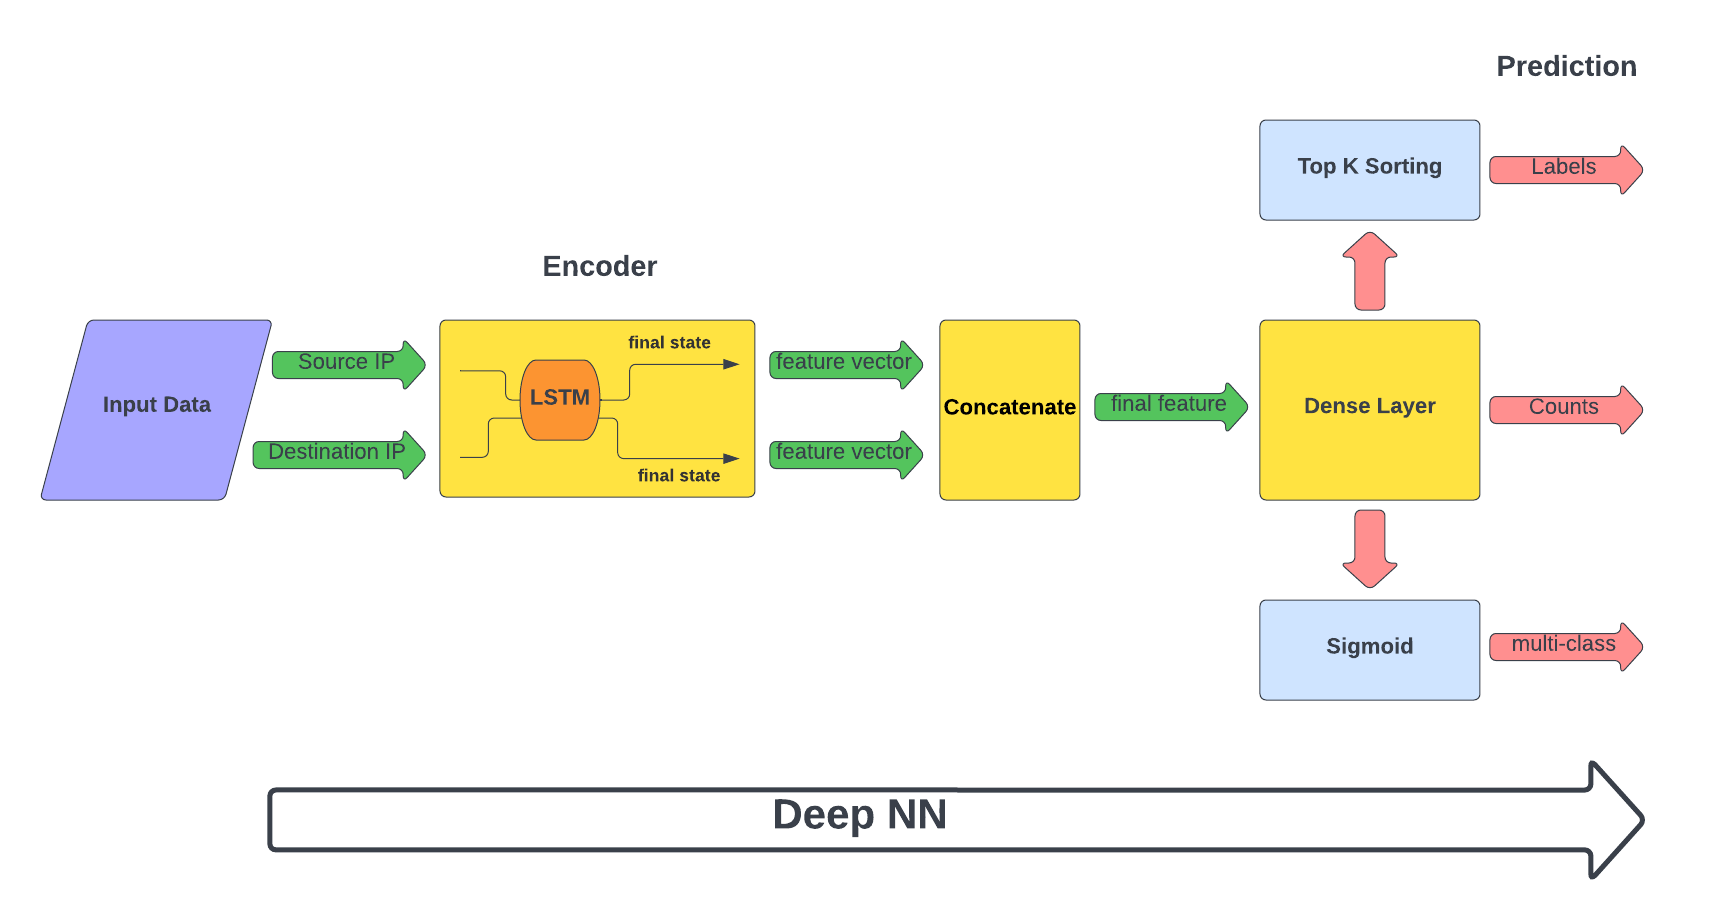
\includegraphics[width=1\textwidth]{images/workflow/learned oracle(4).png}
\caption{Overview of the Learned Oracle workflow.}
\label{fig:ml_flow}
\end{figure}

We train a neural network to predict the log of the packet counts for each flow. 

In Figure~\ref{fig:ml_flow}, we can see our ML workflow. The model is fed the IP addresses contained in each packet as input. We encode the source and destination IP addresses independently using two RNNs. At each step, the RNN extracts one bit of the IP address, beginning with the most important bit. We employ the RNN's final states as the feature vector for an IP address. The reason for using RNN is that the bit patterns are hierarchical, i.e., the more significant bits regulate greater parts of the IP space. Then, as final features, we concatenate the encoded IP addresses to predict the packet counts. 

In addition, to make the model more versatile and robust, we add two more output options into the network. By doing so, we are able to alternate or combine with different outputs and apply different loss functions for updating the network and metrics for evaluations. One of them is top k sorting: it takes the predicted counts as input, sorts them by descending order and labels them with 1 or 0 by comparing them with the k-threshold value. The other one is sigmoid activation layer. This layer transforms the previous predicted counts into probabilities of belonging to 'top' and 'bottom', i.e., multi-class classification.

\subsection{Importance-based Learning Flow}

Depicted in Figure~\ref{fig:relabel_flow} is a visualization of our semi-supervised model workflow using relabeling. The design makes use of an oracle HH(i) to ascertain whether an item i is a "heavy hitter". Each item categorized as heavy hitter is placed into one of the $B_{r}$ unique buckets designated for them. All remaining $B - B_{r}$ items are distributed across the remaining buckets using a standard frequency estimation technique like Count-min Sketch. 

Analogous procedures apply to count estimating. To calculate $\tilde{f}_i$, the algorithm first verifies if an item i is kept in a unique bucket and, if it is, it returns its count. Otherwise, Count-min is queried. Please be aware that if the element is placed in a unique bucket, the count returned is genuine, that is, $\tilde{f}_i = f_i$.

The oracle is built using machine learning techniques and trained on a small chunk of the data stream S, named as $S'$.
Take note that the oracle learns the properties that distinguish heavy hitters, not their identities. For instance, the oracle would learn that shorter words are more commonplace, allowing it to recognize popular words even when they were not included in the training set $S'$. 

\begin{figure}[htbp!]
\centering
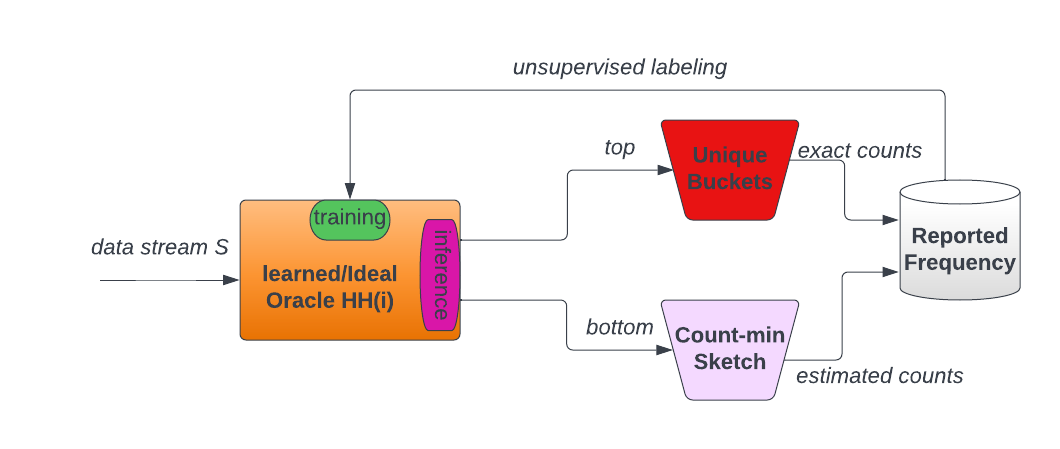
\includegraphics[width=\textwidth]{images/workflow/relabeling.png}
\caption{Relabeling using output of Sketch}
\label{fig:relabel_flow}
\end{figure}

Besides implementing supervised learning using subset $S'$ with correct labels, we utilize some datasets without labels. In Figure~\ref{fig:relabel_flow}, we use the ideal oracle to draw inferences from these unlabeled data, then feed the prediction to the unique buckets or Sketch as we discussed to get the reported counts, also named as pseudo-labels. We send these pseudo-labels(output of the whole system) back to the oracle for continue training. By doing so, we integrate supervised learning and unsupervised learning together, that is, semi-supervised learning.


\subsection{Adaptive Learning Flow}


\begin{figure}[htbp!]
\centering
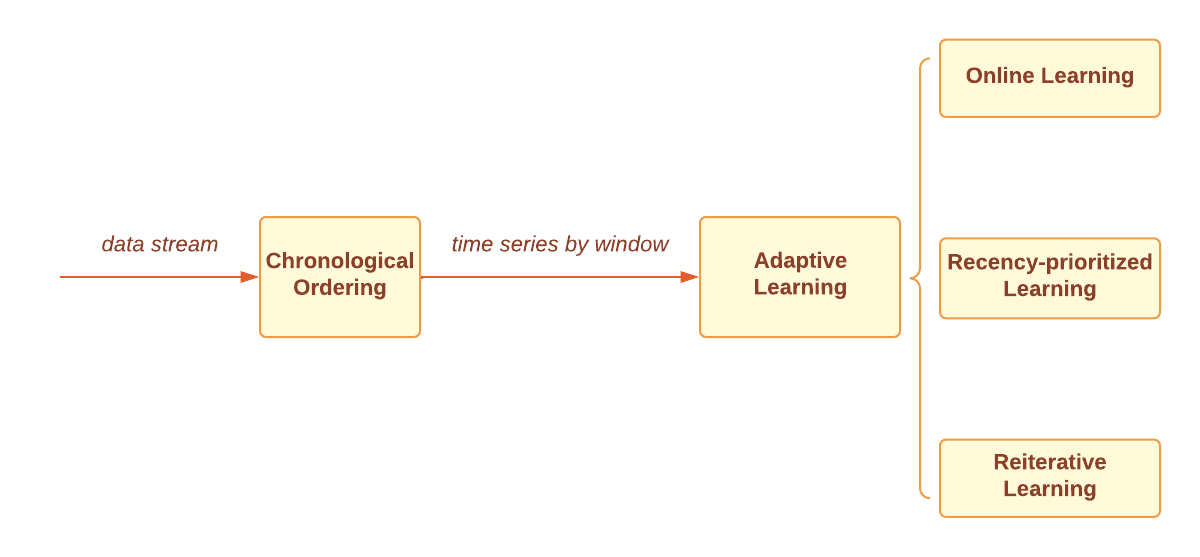
\includegraphics[width=\textwidth]{images/workflow/adaptive learning.png}
\caption{Adaptive Learning on Chronological Data }
\label{fig:adaptive_flow}
\end{figure}

Firstly, we do data preprocessing so that we bring data stream in a chronological order. We read data from file: 8 bytes for timestamp, 4 bytes for source IP, 4 bytes for destination IP. After that, we extract data from window (based on value of timestamp) out of dataset, separate data into windows of predefined length, and write all windows row-wise being chronological dataset. In the end, we take out the 1000 most frequent flows with their total occurrences as preprocessed dataset.

% adaptive learning
To address concept drift, as depicted in Figure~\ref{fig:adaptive_flow}, we decide to apply the following adaptive learning techniques:

\begin{enumerate}
    \item \emph{Online learning~\cite{lee2020clinical}} Instead of learning on the entire training data set at once, we additionally update the model at each temporal step from our preprocessed sequential data. By doing so, the learned oracle dynamically adapts to new patterns in the data.
    
    \item \emph{Recency-prioritized learning} There is a need to optimize the trade-off between offline and online learning. We pick latest batches with a higher likelihood, therefore the model is aware of recent patterns while the training is still extensive.

    
    \item \emph{Reiterative learning~\cite{liang2018weakly}} Whenever the model has become too outdated (criteria of which would be up to the meta-learning part of the model to determine), we perform further learning.

\end{enumerate}

\subsection{Top k Pyramid Flow}

After feature tensors pass through RNN layers, instead of solely utilizing dense layers to predict the counts, we add our custom-built pooling layers alternated with deep layers.

\begin{figure}[htbp!]
\centering
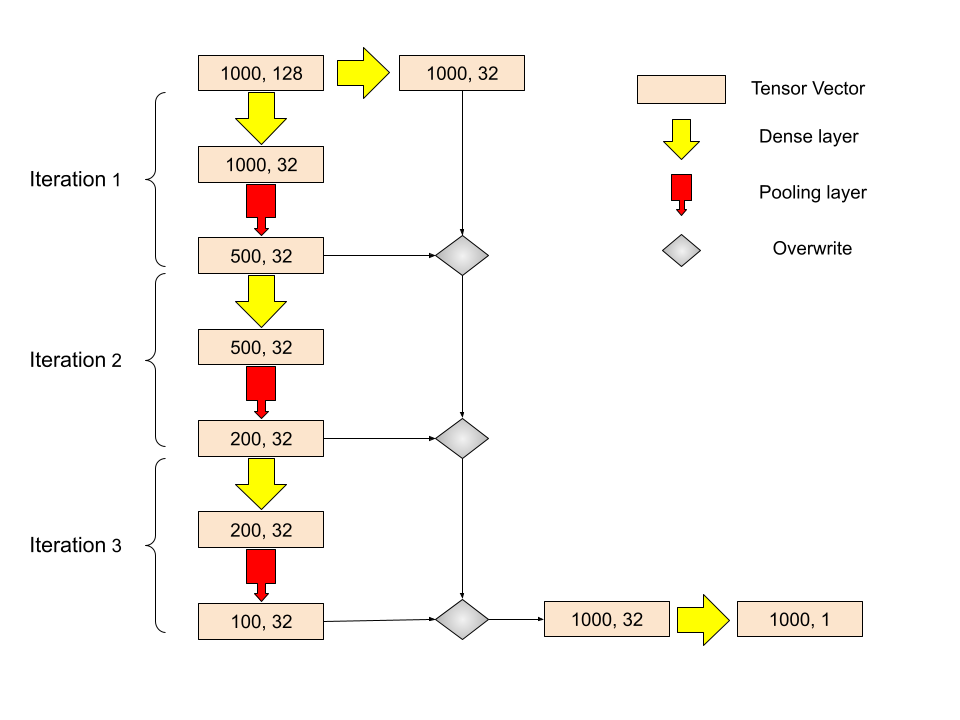
\includegraphics[width=\textwidth]{images/workflow/topk_pyramid.png}
\caption{Pyramid of top-k pooling alternated with dense layers}
\label{fig:topk_pyramid}
\end{figure}

As shown in Figure~\ref{fig:topk_pyramid}, in the very beginning, we branch out the input tensor, apply a dense layer of 32 units and get the output as the preparatory sequence for later overwriting usage. Afterwards, in each iteration, a dense layer is followed by a pooling layer. Our custom-designed pooling layer consists of the following steps:

\begin{enumerate}
    \item \emph{Regress} We apply a full-connected layer with 1 unit. By doing so, we are able to change the second dimension of the input tensor from 32 to 1.
    
    \item \emph{Sort and obtain indices} Now that we obtain a tensor of dimension (batch size,1), we sort this tensor by descending order of values from its second dimension and fetch indices of the top k elements. The value of k decreases after each iteration ends.  

    \item \emph{Extract relevant sequence} Having the top k indices, we map these indices back to the initial input sequence of the pooling layer, and extract corresponding elements we desire. Then, we use the activation function to get the output as the input for the next iteration as well as cache for later use.

\end{enumerate}

Our model contains three iterations, that is to say, we pool three times from the starting sequence with three different values of k and also get three intermediate pooled sequences as caches.

We utilize the cache we get from each iteration in order and overwrite the preparatory sequence so that  we integrate information of top elements in the output sequence. In the end, we add a 1-unit dense layer to predict the counts.
